
\cleardoublepage

\noindent{\bf\Huge\color{oblue} Executive summary}
\addcontentsline{toc}{chapter}{Executive summary}
\vspace{1cm}



\begin{minipage}{0.5\textwidth}

\includegraphics[width = 0.8\textwidth]{recruitement_problem.jpg}
\end{minipage} \hfill
\begin{minipage}{0.45\textwidth}
\noindent{\bf\huge\color{oyellow} The problem}
\medskip

\noindent You need to find the best candidate for a 
job offer, in a increasingly digitized environment.
Could you use the information contained in social networks
to optimize the process?
\end{minipage}
\vspace{1.5cm}


\begin{minipage}{0.7\textwidth}
\noindent {\bf\huge\color{oyellow} A new information source:\newline\noindent Twitter}
\medskip

\noindent We will retrieve published tweets
with content related to the job offer, and then use our innovative
algorithms to:
\begin{itemize}
\item identify tweets languages,
\item select the tweets by the relevance of its contents,
and extract the active users with the required profile,
\item propose the outstanding candidates for the job offer.
\end{itemize}
\end{minipage}\hfill
\begin{minipage}{0.4\textwidth}
\begin{tabular}{c}

\includegraphics[width=0.4\textwidth]{twitter-logo-final.png}\\

\includegraphics[width=0.2\textwidth]{flecha.pdf}\\
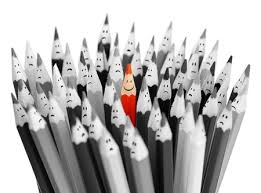
\includegraphics[width=0.8\textwidth]{rightcandidate.jpg}
\end{tabular}
\end{minipage}
\vspace{1.5cm}


\begin{minipage}{0.4\textwidth}
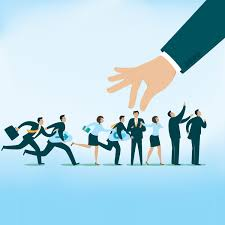
\includegraphics[width=0.8\textwidth]{candidate_selection.jpg}
\end{minipage}\hfill
\begin{minipage}{0.55\textwidth}
{\bf\huge\color{oyellow} Which are the best candidates?}
\medskip

\noindent We use two different ordering algorithms to
rank the list of the candidates and find the best ones:
\begin{itemize}
\item By published contents: $h$-index
\item By relevance in the users network: centrality measures (degree, eigenvector,
 Bonacich, PageRank, closedness, betweenness).
\end{itemize}
\noindent Go to Shiny to navigate the ordered list!
\end{minipage}




\begin{sidewaysfigure}
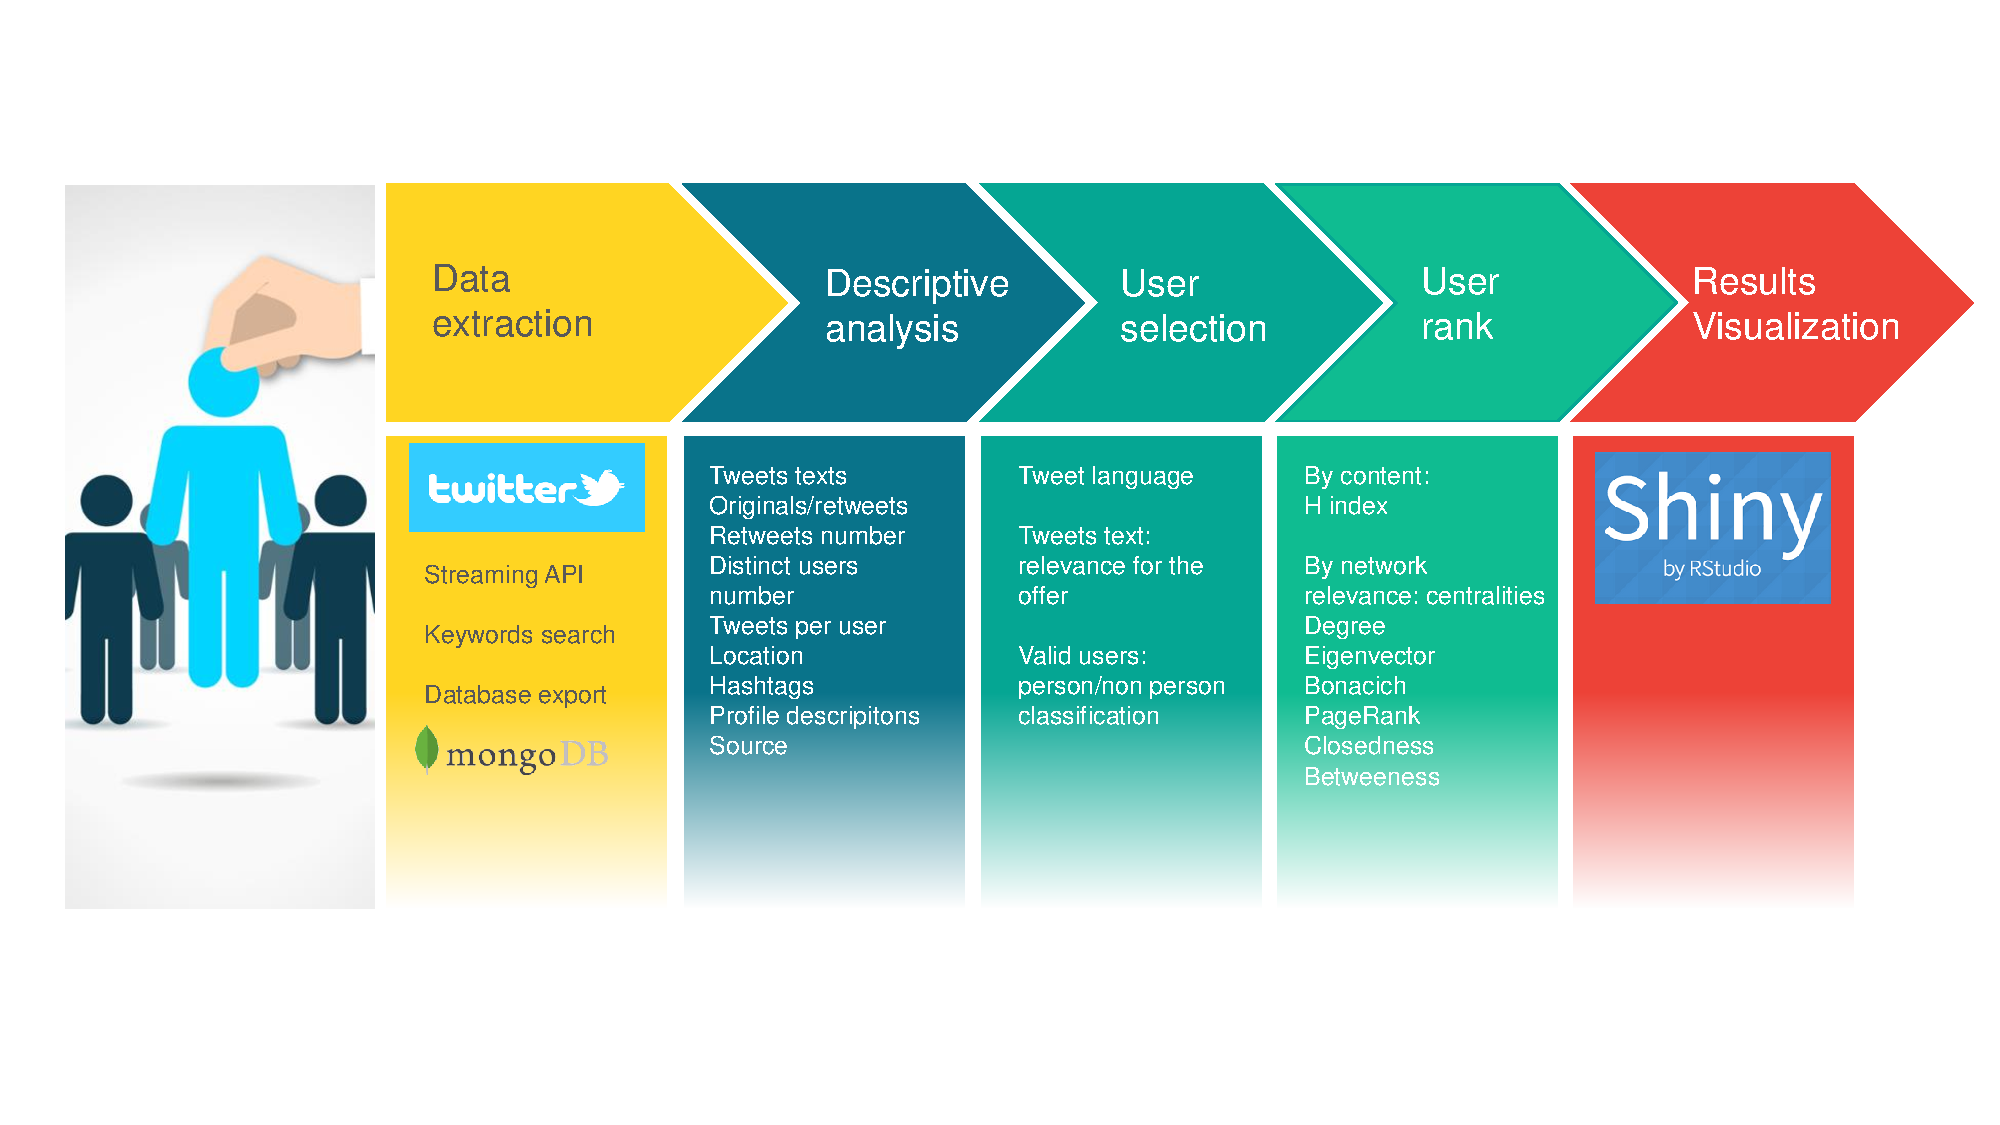
\includegraphics[width=\textwidth]{workflow_eng.pdf}
\caption{Schematic workflow.}
\label{fig:workflow}
\end{sidewaysfigure}